% !Mode:: "TeX:UTF-8"
%!TEX program  = xelatex

\documentclass{cumcmthesis}
\usepackage{graphicx}
\usepackage{float}
\usepackage{subfig}
\usepackage{footnote}
\usepackage{mathrsfs}
\usepackage{algorithm}
\usepackage{algorithmicx}
\usepackage{algpseudocode}
\usepackage{amsmath}
\usepackage{xcolor}
\usepackage{booktabs}
\usepackage{dcolumn}
\usepackage[sort&compress]{gbt7714}
\usepackage{tikz}
\usetikzlibrary{shapes.geometric, arrows}
\tikzstyle{startstop} = [rectangle, rounded corners, minimum width = 2cm, minimum height=1cm,text centered, draw = black]
\tikzstyle{io} = [trapezium, trapezium left angle=70, trapezium right angle=110, minimum width=2cm, minimum height=1cm, text centered, draw=black]
\tikzstyle{process} = [rectangle, minimum width=3cm, minimum height=1cm, text centered, draw=black]
\tikzstyle{decision} = [diamond, aspect = 3, text centered, draw=black]
\tikzstyle{arrow} = [->,>=stealth]

\definecolor{mygreen}{rgb}{0,0.6,0}
\definecolor{mygray}{rgb}{0.5,0.5,0.5}
\definecolor{mymauve}{rgb}{0.58,0,0.82}
\lstset{ %
	backgroundcolor=\color{white},      % choose the background color
	basicstyle=\footnotesize\ttfamily,  % size of fonts used for the code
	columns=fullflexible,
	tabsize=4,
	breaklines=true,               % automatic line breaking only at whitespace
	captionpos=b,                  % sets the caption-position to bottom
	commentstyle=\color{mygreen},  % comment style
	escapeinside={\%*}{*)},        % if you want to add LaTeX within your code
	keywordstyle=\color{blue},     % keyword style
	stringstyle=\color{mymauve}\ttfamily,  % string literal style
	frame=single,
	rulesepcolor=\color{red!20!green!20!blue!20},
	% identifierstyle=\color{red},
	language=C++,
}
% \documentclass[withoutpreface,bwprint]{cumcmthesis} %去掉封面与编号页

\usepackage{url}
\title{基于图论模型的核酸检测点设置位置分析}
\tihao{B}
\date{\today}
\usepackage{footnote}

\usepackage{graphicx}
\usepackage{float}
\usepackage{subfig}

\begin{document}

\maketitle

\begin{abstract}

合理地选择核酸检测点的位置可以很大程度上方便居民的核酸检测。本文将小区结构抽象为图结构,对不同的小区中核酸检测点的规划进行了研究,分析核酸检测点位置与人群流动的关系,考虑了多种评价标准与约束条件,对于使总路程和最长路程分别最小的目标分别建立了图论模型。

\textbf{对于问题一}:针对两种目标,笔者先通过枚举核酸检测点所在的边,将原问题转化为单变量优化问题,再经过分析,得出结论:使总路程最小时,核酸检测点一定在点上;使最大路程最小时,核酸检测点在图的绝对中心上。最后,笔者提出了复杂度可以接受的两种算法。

\textbf{对于问题二}:笔者把问题一的结论进行推广,并针对两种目标提出相应的朴素算法。

\textbf{对于问题三}:针对目标一,笔者先建立了整数规划模型,再提出了一种基于模拟退火的智能算法来求出近似最优解。
针对目标二,先用二分法把原问题转化为 Set cover problem(SCP),再针对该问题建立整数线性规划与动态规划模型,由于 Set cover porblem 是 NP-Hard 的,使用了一种随机化的 Greedy 算法来近似地求解该问题,并推导得出了近似解与最优解偏差的一个上界。

最后,笔者分析了不同小区结构对模型的影响,并得出以下结论:

\begin{enumerate}
    \item 核酸检测点趋向于在人口密集处设置;
    \item 当核酸检测点只有一个时,最优解一般在小区中心附近;
    \item 当核酸检测点够多时,最优解一般较为均匀地分布在小区中。
\end{enumerate}


% 未完待续

\keywords{图论\quad  最短路\quad  NP-Hard\quad 模拟退火\quad 整数规划\quad 动态规划}
\end{abstract}

%目录
% \tableofcontents

\section{问题重述}

\subsection{问题背景}

% 2019年冬,新冠病毒疫情席卷全球,对人类的工作,生活等方方面面产生了极大的影响。为了发现病毒携带者,我国使用核酸检测作为发现病毒携带者的的重要手段,执行动态清零政策,进行常态化核酸检测,保障人民安全。核酸检测往往需要大量核酸检测点来支持其采样。为了使居民小区中的核酸检测点设置位置达到最优,方便居民的核酸采样。

% 这也是 bear 写的罢
核酸检测是一种重要且有效的防疫手段。为了保障我国人民群众的生命安全,本着生命至上、人民至上的宗旨,我国采取了动态清零政策进行疫情防控,在有疫情风险的区域进行常态化核酸检测。在核酸检测常态化的背景下,为了方便居民的核酸检测,防疫部门应当科学合理地选择核酸检测点的位置。而由于小区结构的不同,针对不同类型的小区,选择核酸检测点位置的方法是不同的。我们需要找到一系列方法来求出核酸检测点的最优位置。

\subsection{问题提出}

对于不同类型的小区,回答以下问题:

\textbf{问题一}:要求只设立一个检测点,求核酸检测点的最佳位置。

\textbf{问题二}:要求设立两个检测点,求核酸检测点的最佳位置。

\textbf{问题三}:允许设立多个检测点,规划核酸检测点的设置方案。

\section{问题分析}

\subsection{总体分析}

一个居民小区通常由一些单元与道路组成。每个单元都有一定数量的人居住,每条道路都有一定的长度。此外,我们可以把道路的交叉点与空地等看作没有人居住的单元。核酸检测点可以设在单元里,也可以设在道路上。于是我们可以把居民小区抽象为一张连通无向图,以单元为点,点权为居住人数,边权为边的长度,把核酸检测点的规划转化成图论问题进行求解。

定义图上两点的花费为两点的最短路径长度乘上起始点的点权。

建立核酸检测点位置要使居民总体方便,那么建立核酸检测点有两种方案:使得每个人到达核酸检测点的路程和最小或到达核酸检测点的最大的路程最短;并且需要考虑建立的位置是否会给居民的正常生活造成影响。

\section{模型假设}

\begin{enumerate}
    \item 任意两个单元可以通过道路相互到达,即图连通;
    \item 核酸检测点只能设在点上或者边上;
    \item 每一个人都会选择去最近的核酸检测点采样;
    \item 每一个人移动的速度相同;
    \item 不考虑道路堵塞与核酸检测点排队。
\end{enumerate}

\section{符号说明}
\begin{center}
\begin{savenotes}
\begin{tabular}{cc}
\toprule
\makebox[0.3\textwidth][c]{符号}	&  \makebox[0.4\textwidth][c]{意义} \\ \midrule
$n$         & 图的点数 \\
$m$         & 图的边数 \\
$w_i$	    & 第 $i$ 个点的点权 \\
$e_i$	    & 第 $i$ 条边的边权 \\
$u_i$       & 第 $i$ 条边的起点 \\
$v_i$       & 第 $i$ 条边的终点 \\
$d_{i,j}$   & 第 $i$ 个点和第 $j$ 个点最短路径长度 \\
$s_i$       & 第 $i$ 个点的所有人到核酸检测点的距离和 \\
$D$         & 所有人到核酸检测点的总距离和 \\ \bottomrule
\end{tabular}
\end{savenotes}
\end{center}

\section{模型建立与求解}

\subsection{问题一}

假设核酸检测点在边 $(u_k,v_k)$ 上,设其距 $u_k$ 的距离为 $x(x \in [0,e_k])$,那么它距离 $v_k$ 的距离为 $e_k - x$。对于一个节点 $i$,
第 $i$ 个节点的人到核酸检测点的最短路程为 $\min\left\{d_{u_k,i}+x,d_{v_k,i}+e_k-x\right\}$。接下来我们将分别考虑两种评判标准进行求解。

\begin{figure}[H]
    \centering
    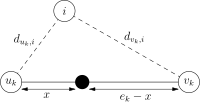
\includegraphics{images/Single-1}
    \caption{核酸检测点与一点的位置关系\upcite{oiwiki-mdst}}
    \label{fig:Single-1}
\end{figure}

\subsubsection{目标一}

使得每一个人到达核酸检测点的路程和最小。

由图可得,点 $i$ 上的人采样所走的最短距离为 $\min\left\{d_{u_k,i}+x,d_{v_k,i}+e_k-x\right\}$,路程和为 $s_i=w_i\cdot\min\left\{d_{u_k,i}+x,d_{v_k,i}+e_k-x\right\}$。

可以发现 $s_i$ 关于 $x$ 的图象一定是一条先升再降的折线或者是直线,因此一定是上凸的。由于每个 $s_i$ 关于 $x$ 是上凸的,所以总路程 $D(x)=\sum_{i=1}^n s_i$ 也是上凸的。
因此得:

\begin{equation*}
    D(x)\ge\min\left\{D(0),D(e_k)\right\}
\end{equation*}

即一定存在一种最优解,使核酸检测点在某个点上。

% $x=\frac{d_{v_k,i}+e_k-d_{u_k,i}}{2}$ 是图象的转折点。

% 可以发现图象一定是一条先升再降的折线或者是直线,因此一定是上凸的。由于每个 $s_i$ 关于 $x$ 是上凸的,所以总路程 $\sum_{i=1}^n s_i$ 也是上凸的。
% 因此 $\sum_{i=1}^n s_i$ 在区间 $[0,e_k]$ 上的最小值一定在 $x=0$ 或 $x=e_k$ 时取到,即核酸检测点一定在某个点上。

以下是算法过程:

\begin{enumerate}
    \item 使用最短路算法求出 $d_{i,j}$;
    \item 枚举每一个点,求出 $\sum_{i=1}^n s_i$,并更新答案。
\end{enumerate}

如果使用堆优化的 Dijkstra 求解最短路,时间复杂度为 $\Theta(n^2\log m)$,若使用 Floyd,时间复杂度为 $\Theta(n^3)$。

\subsubsection{目标二}

使得到达核酸检测点的最长的路程最短。

提出一个概念叫 \emph{图的绝对重心},定义为到所有点的距离的最大值最小的点,那我们的核酸检测点应建立在绝对重心上。

接下来考虑如何求解绝对重心。

假设图的绝对重心在边上,枚举每一条边 $(u_k,v_k)$,钦定图的绝对重心 $c$ 在这一条边上,假设其距 $u_k$ 的距离为 $x(0 \le x \le e_k)$,那么它距离 $v_k$ 的距离为 $e_k - x$。

那么 $d_{c,i} = \min\left\{d_{u_k, i} + x, d_{v_k,i} + e_k - x\right\}$。

随着 $c$ 从 $u_k$ 到 $v_k$ 的移动 $d_{c,i}$ 的变化如图可以画到一个平面直角坐标系上:

\begin{figure}[H]
	\centering
	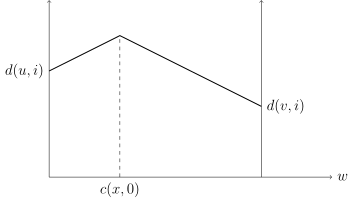
\includegraphics[width=0.6\textwidth,height=0.4\textwidth]{images/mdst-plot1.png}
	\caption{图的绝对中心变化的影响\upcite{oiwiki-mdst}}
	\label{fig:mdst-graph}
\end{figure}

显然可以发现图象会是两条斜率相同的一次函数所构成。

接下来将对于每一个点 $i$ 都画像这样的图象就可以得到:

\begin{figure}[H]
	\centering
	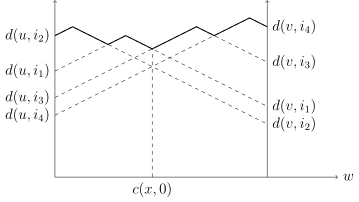
\includegraphics[width=0.6\textwidth,height=0.4\textwidth]{images/mdst-plot2.png}
	\caption{图的绝对中心变化的影响\upcite{oiwiki-mdst}}
	\label{fig:mdst-graph}
\end{figure}

这些折线交点中的最低点,横坐标就是图的绝对中心的位置。

不难发现,出现交点的条件是 $d_{u,i_1} < d_{u,i_2},d_{v,i_1} > d_{v,i_2}$。

对于绝对中心在一个点上,那么就枚举一下那个节点,再用与其距离最远的节点更新一下就行了。

对于每一条边,每一个点都这样做一下就可以了。

总结一下过程:

\begin{enumerate}
    \item 使用最短路算法求出 $d_{i,j}$;
    \item 对于绝对中心在点上更新答案;
    \item 对于绝对中心在边上,枚举每一条边更新答案。
\end{enumerate}

如果使用堆优化的 Dijkstra 求解最短路,时间复杂度为 $\Theta(n^2\log m + nm)$,若使用 Floyd,时间复杂度为 $\Theta(n^3 + nm)$

\subsection{问题二}

\subsubsection{目标一}

可以发现,问题一目标一的结论可以推广到多个核酸检测点。

设第一个核酸检测点在边 $(u_a,v_a)$ 上,到 $u_a$ 的距离为 $x_1$,第二个核酸检测点在边 $(u_b,v_b)$ 上,到 $u_b$ 的距离为 $x_2$。则此处 $D$ 为 $x_1$ 和 $x_2$ 的函数。

我们发现同一个节点的人选择去同一个核酸检测点检测肯定不劣。于是假设节点集合 $S$ 中的人都去第一个核酸检测点采样,$V\setminus S$ 中的人都去第二个核酸检测点采样。令 $D_1(x_1)=\sum_{i\in S}s_i,D_2(x_2)=\sum_{i\in V\setminus S}s_i$。因为 $S\cup (V\setminus S)=V$ 且 $S\cap (V\setminus S)=\emptyset$,所以 $D(x_1,x_2)=D_1(x_1)+D_2(x_2)$。

同问题一可证 $D_1$ 关于 $x_1$ 上凸,$D_2$ 关于 $x_2$ 上凸。因此:

\begin{align*}
    D(x_1,x_2)&=D_1(x_1)+D_2(x_2)\\
    &\ge \min\left\{D_1(0),D_1(e_a)\right\}+\min\left\{D_2(0),D_2(e_b)\right\}\\
    &=\min\left\{D(0,0),D(0,e_b),D(e_a,0),D(e_a,e_b)\right\}
\end{align*}\par

即两个核酸检测点设置在边上时并不能比设在边的端点上更优。该证明同样可以推广到更多核酸检测点的情况。

那只需要枚举两个核酸点,暴力计算取最小值即可。

时间复杂度 $\Theta(n^3)$

\subsubsection{目标二}

这个问题不易求解,不妨钦定核酸检测点不会出现在路上(对于一个小区,设置在路上可能会影响交通,所以对最优性影响不大)。

那么我们只需要同目标一,枚举核酸点,暴力计算取最小值即可。

时间复杂度 $\Theta(n^3)$。

\subsection{问题三}

\subsubsection{目标一}

建立 $k$ 个核酸检测点,使得每一个人到达核酸检测点的路程和最小。

上文已经证明了选择目标一时核酸检测点一定建在图的节点上。于是我们可以提出如下算法。

% 建立优化模型

\paragraph{整数规划解法}

设决策变量为 $x_i$,满足

\begin{equation*}
    x_i=\begin{cases}
    1 & i \text{设立核酸检测点}\\
    0 & \text{其他}
    \end{cases}
\end{equation*}

则可以如下建立规划模型:

\begin{align*}
    &\min\sum_{i=1}^n \left(w_i \min_{x_j=1} d_{i,j}\right)\\
    &\operatorname{s.t.}\begin{cases}\sum_{i=1}^n x_i=k\\x_i\in\{0,1\}\end{cases}
\end{align*}

\paragraph{模拟退火解法}

这个问题笔者未找到复杂度可以接受的精确算法。于是考虑近似算法。在此,我们采用模拟退火算法进行求解。

算法过程如下:

\begin{figure}[H]
    \centering
    \begin{tikzpicture}
        \node[startstop](start){开始};
        \node[process,below of=start,yshift=-0.5cm](init){令温度 $T=T_0$,从 $n$ 个节点中随机选取 $k$ 个作为初始的答案集合 $S$};
        \node[process,below of=init,yshift=-0.5cm](shift){分别在 $S$ 与 $V\setminus S$ 中随机选择节点 $u$ 与 $v$,设 $S'=(S\setminus\{u\})\cup \{v\}$};
        \node[rectangle,right of=shift,xshift=6cm,inner sep=0pt](shift1){};
        \node[rectangle,right of=shift,xshift=6.5cm,inner sep=0pt](shift2){};
        \node[process,below of=shift,yshift=-0.5cm](calc){分别求出在 $S$ 和 $S'$ 设置采样点时的最短总路程 $D$ 与 $D'$};
        \node[decision,below of=calc,yshift=-0.5cm](des1){$D'<D$};
        \node[process,below of=des1,yshift=-0.5cm,xshift=-3cm](accept1){将 $S$ 更新为 $S'$};
        \node[process,below of=des1,yshift=-0.5cm,xshift=3cm](accept2){以 $e^{-\frac{E'-E}{T}}$ 的概率将 $S$ 更新为 $S'$};
        \node[rectangle,below of=accept1,yshift=-0.2cm,inner sep=0pt](accept1d){};
        \node[rectangle,below of=accept2,yshift=-0.2cm,inner sep=0pt](accept2d){};
        \node[decision,below of=accept1d,yshift=-0.5cm,xshift=3cm](des2){是否迭代了 $L$ 次};
        \node[process,below of=des2,yshift=-0.5cm,xshift=3cm](upd){$T=\alpha T$};
        \node[decision,below of=des2,yshift=-1.5cm,xshift=-3cm](des3){$T<T_1$};
        \node[startstop,below of=des3,yshift=-0.5cm](end){结束};
        
        \draw [arrow] (start) -- (init);
        \draw [arrow] (init) -- (shift);
        \draw [arrow] (shift) -- (calc);
        \draw [arrow] (calc) -- (des1);
        \draw [arrow] (des1) -| (accept1);
        \draw [arrow] (des1) -| (accept2);
        \draw (accept1) -- (accept1d);
        \draw (accept2) -- (accept2d);
        \draw [arrow] (accept1d) -| (des2);
        \draw [arrow] (accept2d) -| (des2);
        \draw [arrow] (des2) -| (upd);
        \draw [arrow] (des2) -| (des3);
        \draw [arrow] (des3) -- (end);
        \draw (upd) -| (shift1);
        \draw (des3) -| (shift2);
        \draw [arrow](shift2) -- (shift);
    \end{tikzpicture}
    \caption{问题三目标一流程图}
    \label{fig:3-1-fig}
\end{figure}

经过测试,得到一组较为满意的参数:$T_0=10^9,T_1=0.1,\alpha=0.9,L=5$。为了避免偶然性,可以把这个算法执行 $100$ 次,并取其中的最优解。

下图为多次模拟退火时总距离随迭代次数的变化过程:

\begin{figure}[H]
	\centering
	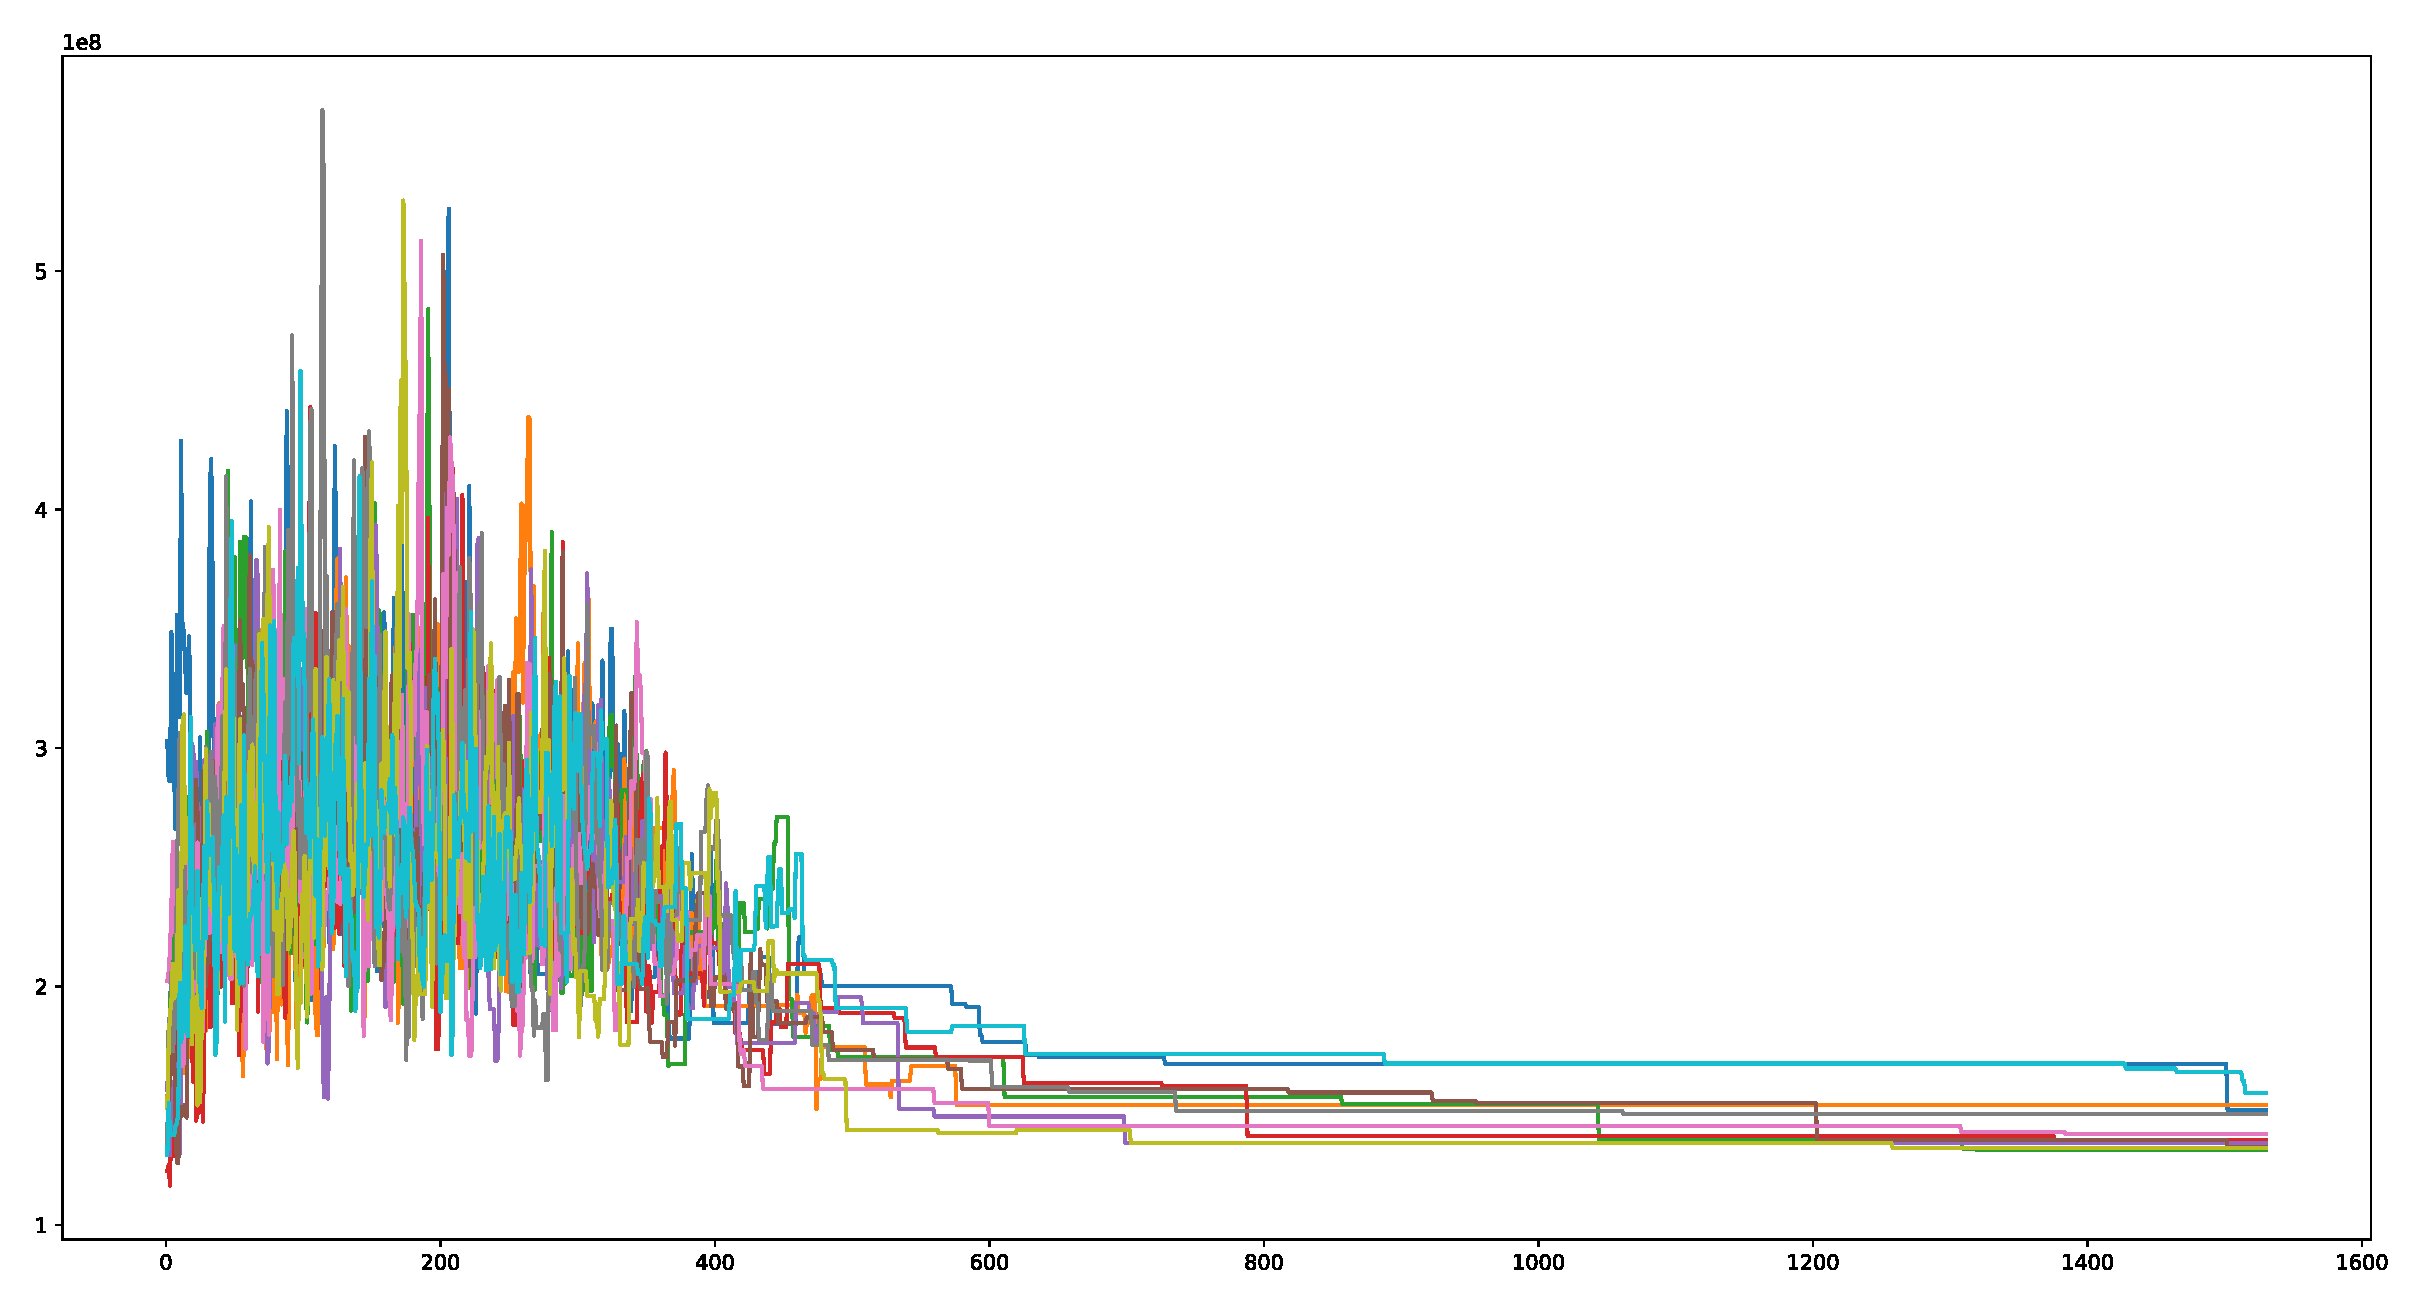
\includegraphics[width=0.80\textwidth]{images/SA.eps}
	\caption{模拟退火求解过程}
	\label{fig:P3T1-SA}
\end{figure}

\subsubsection{目标二}

问题转化为给定一张无向图,在其中选择 $k$ 个点,使得每个点距离其最近的核酸检测点距离最大值最小,同问题二目,不妨钦定核酸检测点在无向图的点上。

发现问题具有单调性,如果每个点距离最近的核酸检测点距离最大值为 $x$ 的时候可行,那么距离最大值大于等于 $x$ 的时候也可行,这一点是显然的。

那么我们可以进行这样的一个过程,初始时 $l=1,r=n$:

\begin{enumerate}
    \item 判定每个点距离最近的核酸检测点距离最大值 $\frac{l+r}{2}$ 是否可行;
    \item 如若可行,那么可将答案变量设为 $\frac{l+r}{2}$,令 $r = \frac{l+r}{2}-1$;
    \item 如若不可行,令 $l = \frac{l+r}{2} + 1$;
\end{enumerate}

对于一个判定,距离最近的核酸检测点距离最大值为 $x$,我们可以将每个点看成一个集合,第 $i$ 个点所对应的集合 $A_i$ 表示到其距离在 $x$ 以内的点集,那么问题转化为:

给定 $n$ 个集合,第 $i$ 个集合记作 $A_i(\forall j \in A_i, j 
\in [1,n])$,从其中选出 $k$ 个集合构成集合 $\mathscr{A}$,试判断是否存在一种选法,使得 $\bigcup\limits_{S \in \mathscr{A}} S = [1,n]$。

经查证,这是一个经典 NP-Hard 问题,集合覆盖问题(Set cover problem,SCP)\upcite{wikipedia-SCP},故精确解只能在非多项式解法中得到,接下来会给出其三种解法,分别为 ILP(整数线性规划),状态压缩动态规划和其近似算法(采用 greedy 算法实现)。

\paragraph{整数线性规划解法}

先求解以下规划问题:

\begin{align*}
    &\min\sum\limits_{S \in \mathscr{A}} X_S\\
    &\operatorname{s.t.}\begin{cases}
        \forall S \in \mathscr{A}, e \in [1,n],\sum_{S;e \in S} x_S \ge 1\\
        \forall S \in \mathscr{A}, X_S \in \{0,1\}
    \end{cases}
\end{align*}

然后判断最优解是否小于等于 $k$,即可判断最长距离是否有可能小于等于阈值。

% 限制:

% \begin{equation*}
% \begin{cases}
% \forall S \in \mathscr{A}, e \in [1,n],\sum_{S;e \in S} x_S \ge 1\\
% \forall S \in \mathscr{A}, X_S \in \{0,1\}
% \end{cases}
% \end{equation*}

% 然后我们需要最小化 $\sum\limits_{S \in \mathscr{A}} X_S$。

\paragraph{状态压缩动态规划解法}

这种做法只能适用于 $n,k$ 较小的情况,即小规模小区。

假设 $f_{i,S,j}$ 表示前 $i$ 个集合,选了 $j$ 个,并集为 $S$(集中,$S$ 第 $i$ 为 $1$ 表示数字 $i+1$ 已经出现过了)。

设 $A_i$ 对应的 $n$ 位二进制数位 $B_i$。

状态转移:

\begin{equation*}
    f_{i,S,j} = \Big ( \bigvee_{S'\vee B_i = S}{f_{i-1,S',j-1}} \Big ) \vee f_{i-1,S,j}
\end{equation*}

初始状态 $f_{0,0,0} = true$。

时间复杂度 $\Theta(nk2^n)$,空间复杂度 $\Theta(nk2^n)$,空间复杂度可使用滚动数组优化到 $\Theta(2^nk)$。

缺点:只可判断,若需给出解法,空间复杂度变为 $\Theta(4^nk)$,所以最后得到距离最近的核酸检测点距离最大值后还需使用其他方法进行构造解。

\paragraph{近似算法}

目前关于集合覆盖问题,仍然找不到一个有效的OPT算法,我们这里提出的是一种基于贪婪策略的近似性算法,算法过程为如下伪代码:

\begin{algorithm}
    \caption{Greedy Set Cover Algorithm}
    \begin{algorithmic}[1]
        \Require 集合 $A_i$
        \Ensure 选择方式
        \State $C \gets \emptyset$
        \State $\mathscr{A} \gets \emptyset$
        \While{$C \neq [1,n]$}
            \State Find the set $A$ whose $|A\setminus C|$ is biggest
            \State $C = C \cup A$
            \State Add $A$ into $\mathscr{A}$
        \EndWhile
        \State \Return $\mathscr{A}$
    \end{algorithmic}
\end{algorithm}

我们每次选取的都是 $|A\setminus C|$ 最大的集合 $A_i$,即每次新添加的集合 $A$ 的覆盖率都是最大的,从而保证局部最优。

此外我们可以通过随机化取优的方法来获得更好的近似效果。具体来说,我们可以进行多次上述算法,每次开始算法前对 $A_i$ 进行一次随机的重排,最终在多个答案中取最优解。

\paragraph{性能分析}

设最优解的答案为 $\mathscr{S}$,$\operatorname{cost_{opt}}X$ 表示此时选择集合 $X$ 的最优解。

在贪婪算法的每次迭代过程中,剩下元素OPT算法的 $cost$ 必定小于等于原问题OPT算法的 $cost$,所以剩余集合平均的 $cost$ 不大于 $\frac{|\operatorname{cost_{opt}}A|}{|[1,n]\setminus C|}$。\footnote{此处 $[1,n]$ 指整数区间 $\mathbb{Z}\cap[1,n]$,下同。}

接着当 $x$ 被覆盖的时候,$|C| \le w$,那么覆盖前 $|[1,n]\setminus C| \ge n - w + 1$。

所以数字 $x$ 被覆盖的平均代价 $\operatorname{price}(x) \le \frac{|\operatorname{cost_{opt}}A|}{n-w+1}$。

设 $H_n=\sum_{i=1}^n\frac 1 i$ 为调和级数前 $n$ 项之和,有 $\sum \operatorname{price}(x) \le (\sum_{i=1}\frac{1}{i}) \cdot \mathscr{S} = H_n \cdot \mathscr{S}$。

于是就证明了这个近似算法得出的 $|\mathscr{A}| \le H_n \cdot \mathscr{S}$。

不可逼近性结果表明,如上的贪婪算法本质上是集合覆盖到低阶项的最佳多项式时间近似算法(Dinur\&Steurer, 2013)通过证明它不能近似于最佳不可近似性来证明最优的不可近似性 ${\displaystyle {\bigl (}1-o(1){\bigr )}\cdot \ln {n}}\text{ 除非 } P{\displaystyle =}NP$,在合理的复杂性假设下。对贪婪算法的更严格的分析表明,近似比正好 ${\displaystyle \ln {n}-\ln {\ln {n}}+\Theta(1)}$。\upcite{greedy-algorithm-for-set-cover}

经实测,该算法求出的答案也较为优秀,会在模型分析中给出实例。

\section{模型分析}

下图为一个较有代表性的小区。它包含人口较为密集的区域(学校)与足够的空地。

\begin{figure}[H]
    \centering
    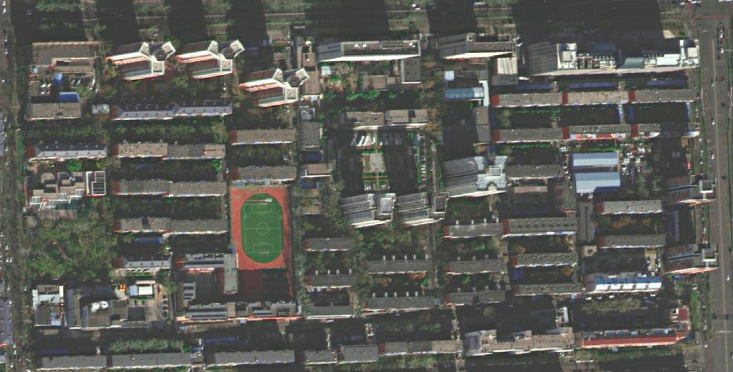
\includegraphics[width=0.8\textwidth]{images/scaled.png}
    \caption{某居民小区}
    \label{fig:scaled}
\end{figure}

将主要的空地和建筑作为节点,相邻节点连边权为几何距离的边(为了方便,以毫米为单位并取整),并设置合理的人口数,得到如下无向图。图中节点大小表示人口多少,空地人口数为 $0$。

\begin{figure}[H]
	\centering
	\subfloat[]{\label{fig:Map}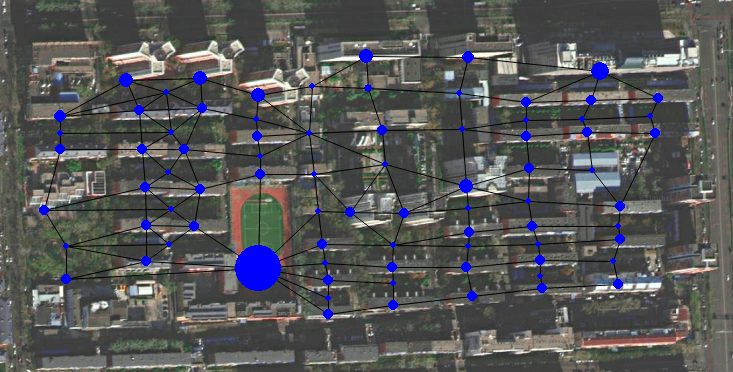
\includegraphics[width=0.6\textwidth]{images/graph-with-map.png}}\\
	\subfloat[]{\label{fig:Graph}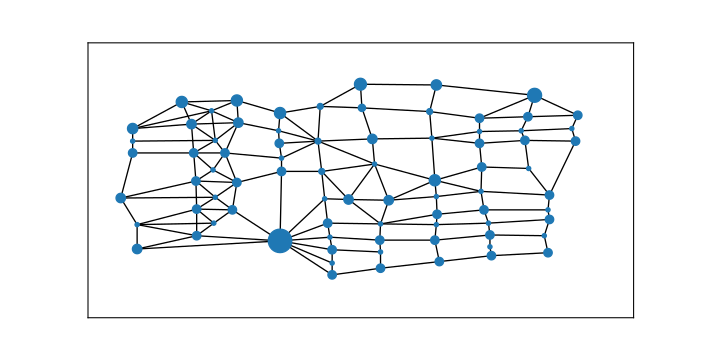
\includegraphics[width=0.8\textwidth]{images/graph.png}}\\	
	\caption{得到的无向图}
\end{figure}

用问题一的程序进行求解并作图(其中红色放大节点是选中的节点)。

\begin{figure}[H]
	\centering
	\subfloat[目标一]{\label{fig:P1T1Ans}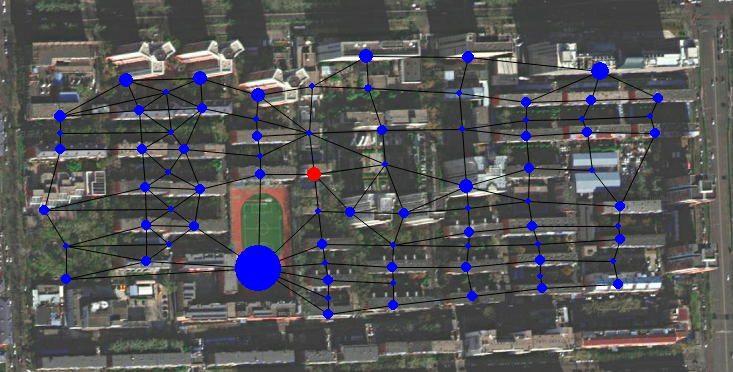
\includegraphics[width=0.6\textwidth]{images/Problem1Subtask1Ans.png}}\\
	\subfloat[目标二]{\label{fig:P1T2Ans}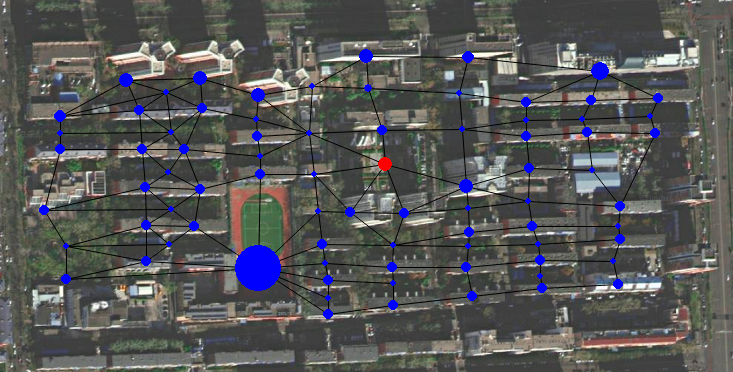
\includegraphics[width=0.6\textwidth]{images/Problem1Subtask2Ans.png}}\\	
	\caption{问题一答案}
\end{figure}

针对目标一求出的解中,人们一共要走 $406.3\mathrm{km}$,总人口为 $2080$ 人,平均每人只要走 $195.4\mathrm{m}$。针对目标二求出的解中,人们最长要走 $366.4\mathrm{m}$。

可以发现,目标一与目标二下的最优解大致都位于小区中心处,且二者距离不大。\newpage

用问题三的程序进行求解并作图,其中 $k=5$。

\begin{figure}[H]
	\centering
	\subfloat[目标一]{\label{fig:P3T1Ans}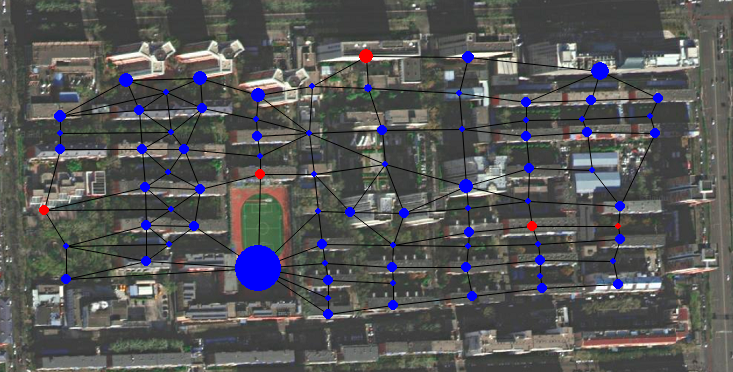
\includegraphics[width=0.6\textwidth]{images/Problem3Subtask1.png}}\\
	\subfloat[目标二]{\label{fig:P3T2Ans}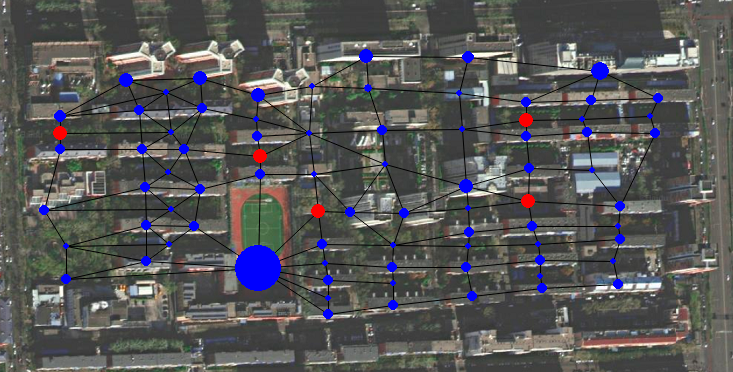
\includegraphics[width=0.6\textwidth]{images/Problem3Subtask2.png}}\\	
	\caption{问题三答案}
\end{figure}

可以发现,虽然两种方案存在较大差别,但是核酸检测点的分布都相对均匀。

\newpage
如下是一张计算机生成的网格图,人口疏密不一。

\begin{figure}[H]
	\centering
	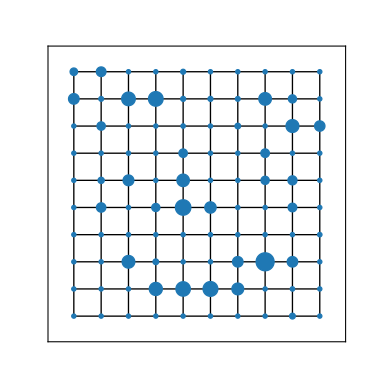
\includegraphics[width=0.6\textwidth]{images/graph_Face.png}
	\caption{网格图}
\end{figure}

用问题三的程序求解得:

\begin{figure}[H]
	\centering
	\subfloat[目标一]{\label{fig:P3T1AnsF}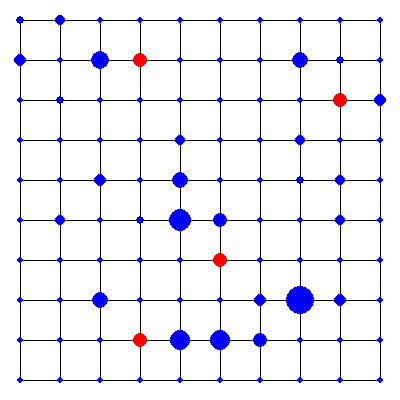
\includegraphics[width=0.3\textwidth]{images/Problem3Subtask1F.png}}
	\subfloat[目标二]{\label{fig:P3T2AnsF}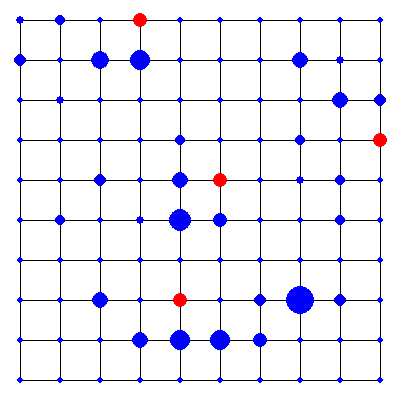
\includegraphics[width=0.3\textwidth]{images/Problem3Subtask2F.png}}\\	
	\caption{问题三答案}
\end{figure}

针对目标一求出的解中,核酸检测点基本分布在人数较多的区域,使得总路程更小;针对目标二求出的解中分布较为均匀,虽然不是最优解,但能保证每个人走过的路程都较短。

\section{模型评价与改进}

\subsection{优点}

可以给出一组较为精确的解。在实际应用的时候,可以将目标一二相结合,如交错选取,$k$ 个检测点一半选择目标一,一半选择目标二,或是则优选取,使用目标一的答案计算所有点到核酸检测点的路径长度和,使用目的答案计算离核酸检测点最远的点的路径长度,而后两者比较和对方的差异,择优选取。

并且还具有模型的计算速度比较快的优点,基本对于现在我国现有的小区规模甚至社区规模都可以在很快的时间内进行计算,算法容易扩展,可以加上各种各样的限制,比如可以在有些点不能建立核酸检测点的时候仍找到一组较为优秀的解。

\subsection{不足}

模型未考虑有关道路情况、核酸检测点排队等问题。在实际生活中,核酸检测点大多不为一整天开放,基本在大部分人上班前、下班后进行检测,短时间内去做核酸的人极多,可能造成排队阻塞交通等问题。所以在确定下有一组答案后,可采用程序模拟检测的情况,并结合人工调节来得到更为优秀的核酸监测点位置。模型较为理想化,但实际生活中难以找到这样理想化的情况。

改进可给每条边设上一个人流限制,也就是人流达到怎样的时候会发生堵塞,然后再保证减少堵塞的情况下利用费用流模型求解。

\subsection{总结}

虽有不足,但笔者在真实出现的小区上的测试,均得到了较为满意的答案,确实满足了绝大部分人的利益,并保证基本所有人不会感到不公平。

\newpage
\bibliographystyle{gbt7714-numerical}
\bibliography{ref}
\newpage

%附录
\begin{appendices}


\section{问题一目标一代码}

\begin{lstlisting}
#include <iostream>
using namespace std;
typedef long long ll;
const ll INF = 1e18;

int N, M;
ll G[510][510], Dist[510][510], Rank[510][510], W[510];

void Center_Point(int &u, int &v, double &x) {  // 返回值为绝对中心在边 $(u,v)$,与 $u$ 的距离为 $x$
    for (int k = 1; k <= N; k++) {
        for (int i = 1; i <= N; i++) {
            for (int j = 1; j <= N; j++) {
                Dist[i][j] = min(Dist[i][j], Dist[i][k] + Dist[k][j]);
            }
        }
    }

    for (int i = 1; i <= N; i++) {
        for (int j = 1; j <= N; j++) Rank[i][j] = j;
        for (int j = 1; j <= N; j++) {
            for (int k = j + 1; k <= N; k++) {
                if (Dist[i][Rank[i][j]] > Dist[i][Rank[i][k]]) {
                    swap(Dist[i][Rank[i][j]], Dist[i][Rank[i][k]]);
                }
            }
        }
    }

    double Ans = 1e18;
    for (int i = 1; i <= N; i++) Ans = min(Ans, Dist[i][Rank[i][N]] * 2.00);
    for (int i = 1; i <= N; i++) {
        for (int j = 1; j <= N; j++) {
            if (i == j || G[i][j] == INF) continue;
            int p = Rank[i][N];
            ll Temp = W[i] * Dist[i][p];
            if (Ans > Temp) {
                Ans = Temp;
                u = i;
                v = j;
                x = 0.00;
            }
            for (int k = N - 1; k >= 1; k--) {
                int t = Rank[i][k];
                if (Dist[j][t] > Dist[j][p]) {
                    Temp = (Dist[i][t] + Dist[j][p] + G[i][j]);
                    if (Ans > Temp) {
                        Ans = Temp;
                        u = i;
                        v = j;
                        x = (Dist[j][p] + Dist[i][j] - Dist[i][t]) / 2.00;
                    }
                    p = t;
                }
            }
        }
    }
    return;
}
\end{lstlisting}

\section{问题一目标二代码}

\begin{lstlisting}
#include <iostream>
using namespace std;
typedef long long ll;
const ll INF = 1e18;

int N, M;
ll G[510][510], Dist[510][510], Rank[510][510], W[510];

int Solve() { // 返回核酸检测点位置
    for (int k = 1; k <= N; k++) {
        for (int i = 1; i <= N; i++) {
            for (int j = 1; j <= N; j++) {
                Dist[i][j] = min(Dist[i][j], Dist[i][k] + Dist[k][j]);
            }
        }
    }

    int ans=0;ll r=INF;
    for(int i = 1; i <= N; i++){
        ll t=0;
        for(int j = 1;j <= N; j++){
            t += Dist[i][j] * W[j];
        }
        if(t<r) ans = i, r = t;
    }

    return ans;
}
\end{lstlisting}

\section{问题三目标一代码}

\begin{lstlisting}
#include <bits/stdc++.h>
using namespace std;
typedef long long ll;
const ll INF = 1e18;

const double T0 = 1e9, T1 = 0.1, a = 0.9;
const int L = 5, T = 100;

ifstream GIn("Graph.txt");
ofstream Ans("Ans.txt");
ofstream Log("Log.txt");

mt19937 mt;
int Rnd(int L, int R) {
    return L + mt() % (R - L + 1);
}
uniform_real_distribution<double> U(0, 1);

ll G[510][510], Dist[510][510], W[510];

int n, m, k;
int p[510];

ll ans = INF;
int ansp[510];

multiset<ll> g[510];

void add(int u) {
    for (int i = 1; i <= n; i++) {
        g[i].insert(Dist[i][u]);
    }
}
void del(int u) {
    for (int i = 1; i <= n; i++) {
        g[i].erase(Dist[i][u]);
    }
}
ll calc() {
    ll r = 0;
    for (int i = 1; i <= n; i++) {
        r += W[i] * (*g[i].begin());
    }
    return r;
}

void Solve() {
    for (int i = 1; i <= n; i++)
        for (int j = 1; j <= n; j++)
            Dist[i][j] = G[i][j];
    for (int k = 1; k <= n; k++)
        for (int i = 1; i <= n; i++)
            for (int j = 1; j <= n; j++)
                Dist[i][j] = min(Dist[i][j], Dist[i][k] + Dist[k][j]);

    for (int i = 1; i <= n; i++) p[i] = i;
    shuffle(p + 1, p + n + 1, mt);

    double T = T0;
    for (int i = 1; i <= k; i++) add(p[i]);
    ll D = calc();
    while (T > T1) {
        for (int t = 1; t <= L; t++) {
            int &u = p[Rnd(1, k)];
            int &v = p[Rnd(k + 1, n)];
            add(v);
            del(u);
            ll r = calc();
            if (r < D || (U(mt) < exp(-(r - D) / T))) {
                D = r;
                swap(u, v);
            } else {
                add(u);
                del(v);
            }
            Log << D << "\n";
            if (D < ans) {
                ans = D;
                for (int i = 1; i <= k; i++) ansp[i] = p[i];
            }
        }
        T *= a;
    }
    fill(p + k + 1, p + n + 1, 0);
}

int main() {
    mt.seed(chrono::system_clock::now().time_since_epoch().count());

    GIn >> n >> m >> k;
    for (int i = 1; i <= n; i++) GIn >> W[i];
    for (int i = 1; i <= n; i++)
        for (int j = 1; j <= n; j++)
            if (i != j) G[i][j] = INF;
    for (int i = 1; i <= m; i++) {
        int u, v;
        ll w;
        GIn >> u >> v >> w;
        G[u][v] = w;
        G[v][u] = w;
    }

    for (int i = 1; i <= T; i++) Solve();
    cout << ans << endl;

    for (int i = 1; i <= k; i++) {
        Ans << ansp[i] << " ";
    }
    Ans << "\n";

    return 0;
}
\end{lstlisting}

\section{问题三目标二代码}

\begin{lstlisting}
#include <bits/stdc++.h>
using namespace std;
const int MAXN = 510;

int N, M, K;
bitset<MAXN> A[MAXN], U;
long long W[MAXN];
long long G[MAXN][MAXN];
int Id[MAXN];
bitset<MAXN> Ans;

bool Check(long long x) {
    for (int i = 1; i <= N; i++) {
        Id[i] = i;
    }
    vector<int> S;
    bitset<MAXN> C;
    for (int i = 1; i <= N; i++) A[i].reset();
    random_shuffle(Id + 1, Id + 1 + N);
    for (int i = 1; i <= N; i++) {
        for (int j = 1; j <= N; j++) {
            if (W[i] * G[Id[i]][j] <= x) {
                A[Id[i]][j] = true;
            }
        }
    }
    while (C != U) {
        pair<int, int> Max = {0, 0};
        for (int i = 1; i <= N; i++) {
            int x = 0;
            for (int j = 1; j <= N; j++) {
                if (A[Id[i]][j] == 1 && C[j] == 0) {
                    x++;
                }
            }
            if (x > Max.first) {
                Max = {x, Id[i]};
            }
        }
        C = C | A[Max.second];
        S.push_back(Max.second);
        if (S.size() > K) return false;
    }
    Ans.reset();
    for (int i : S) Ans[i] = true;
    return true;
}

int main() {
    srand(time(0)); 
    scanf("%d %d %d", &N, &M, &K);
    memset(G, 0x3f, sizeof G);
    for (int i = 1; i <= N; i++) {
        scanf("%d", &W[i]);
        W[i]++;
        G[i][i] = 0;
        U[i] = true;
        Id[i] = i;
    }
    for (int i = 1; i <= M; i++) {
        static int u, v, w;
        scanf("%d %d %d", &u, &v, &w);
        G[u][v] = w;
        G[v][u] = w;
    }
    for (int k = 1; k <= N; k++) {
        for (int i = 1; i <= N; i++) {
            for (int j = 1; j <= N; j++) {
                G[i][j] = min(G[i][k] + G[k][j], G[i][j]);
            }
        }
    }
    long long l = 1, r = 0;
    for (int i = 1; i <= N; i++) {
        for (int j = 1; j <= N; j++) {
            r = max(r, W[i] * G[i][j]);
        }
    }
    while (l <= r) {
        long long mid = l + r >> 1;
        if (Check(mid))
            r = mid - 1;
        else
            l = mid + 1;
    }
    for (int i = 1; i <= N; i++) {
        if (Ans[i]) {
            cout << i << " ";
        }
    }
    return 0;
}
\end{lstlisting}

\end{appendices}

\end{document} 